\chapter{Modèle} \label{ch:modele}

Le modèle cherche à simuler la propagation de pandémies dans une population. Le système inclut des acteurs qui peuvent faire des actions ainsi qu'un **espace physique** sur lequel les acteurs peuvent se déplacer. Les acteurs sont des organismes vivants qui se déclinent en deux espèces distinctes. Le premier groupe fait partie des organismes victimes de l'épidémie et le second groupe est responsables de l'infection. Par conséquent nous sommes dans une situation ou une espèce en attaque une autre. Par contre dans le fonctionnement du modèle, il y a des restrictions sur la nature de l'espèce attaquante. Nous parlons ici d'organismes capables de contaminer un hôte. \\

Les organismes évoluent dans une monde plat et parfaitement géométrique en deux dimensions. L'espace est comparable à un échiquier avec les acteurs étant des pions.

\section{Acteurs}

Il existe exclusivement deux espèces d'organismes dans le système :\\

Les agents pathogènes sont les agents infectieux responsable de l'épidémie.\\
Les hôtes potentiels, éléments de la population victime de l'épidémie.\\

La classe "agents pathogènes" ne fait pas référence à une espèce en particulier mais reflète des organismes avec le pouvoir d'infecter une autre espèce. Il peut s'agir de virus, bactéries ou encore parasites. La caractéristique de ce groupe est qu'il a le pouvoir de rendre malade un hôte et donc d'affecter une espèce par une maladie qu'il génère. Il peut s'agir de maladies touchant des humain ou de zoonoses suivant la nature des espèces du système. Le terme "pathogène" est aussi utilisé pour caractériser cette classe.\\

Les "Individus" sont les organismes susceptible de développer la maladie suite à la contamination par un agent pathogène. Il peut s'agir d'humains tout comme d'animaux ou de plantes. La restriction est que cette espèce doit être affectée par les agents pathogènes ainsi que par la maladie. Le terme "hôte potentiel" signifie que l'organisme peut devenir l'hôte de l'agent pathogène. Nous parlons de "hôte du pathogène" ou de "hôte contaminé" lorsque l'organisme est contaminé et porteur de l'agent pathogène. Le travail utilise souvent le mot "individu" et ceci pour représenter un acteur de ce groupe. Le fait que l'individu soit sain ou contaminé est toujours précisé.

\subsection{Individus}

Un individu peut se présenter sous deux formes distinctes. Il est soit sain, soit contaminé par un agent pathogène.\\

Le premier cas représente un hôte potentiel qui n'est pas contaminé par un agent pathogène et donc n'est pas touché par la maladie. Contrairement à ce que l'on pourrait penser, l'illustration ne fait pas référence à un humain mais à un individu potentiellement vulnérable à la classe des agents pathogènes.\\

Le second cas fait référence à la même espèce mais cette fois ci, l'individu est contaminé par un agent pathogène. Le modèle ne fait pas la distinction entre malade et porteur du virus. Par conséquent, un hôte porteur du pathogène est d'office considéré comme malade. De plus, le modèle définit un taux de contagion qui est paramétrable. Le niveau de contagion est donc constant pour tous les organismes contaminés et ceci tout du long de la simulation. Un hôte infecté par un agent pathogène est donc contagieux, ce qui signifie qu'il a la pouvoir de transmettre l'agent pathogène à d'autres individus de la même espèce. Tout comme pour le point précédent, l'illustration ne fait pas forcément référence à un humain.

\subsection{Agents pathogènes}

Un agent pathogène peut se présenter sous deux formes distinctes. Il est soit contaminant un hôte, soit contaminant un espace physique.\\

Le premier cas est identique à celui précédemment développé mais cette fois ci, la situation est perçue du point de vue de l'agent pathogène. Quand un hôte devient contaminé par un agent pathogène, ce dernier est absorbé par l'hôte. C'est-à-dire que l'agent pathogène n'est plus une entité distincte mais fait partie intégrante de l'individu. Par conséquent l'individu devient un hôte contaminé et non pas un hôte sain associé à un agent pathogène.\\

Le second cas indique qu'une surface physique est contaminée par un agent pathogène. Un hôte contaminé, en plus de contaminer d'autres individus sains, peut contaminer une surface. Si une surface est contaminée, une copie de l'agent pathogène de l'hôte se dépose sur la surface. Un agent pathogène qui contamine une surface est inerte, c'est-à-dire qu'il ne peut pas se déplacer ni muter par contre il a toujours le potentiel de contaminer des individus sains qui se trouveraient sur cette surface. Un agent pathogène isolé sur une surface ainsi n'a une durée de vie que très limitée. Sa chance survie est paramétrable dans le modèle.

\section{Espace physique}

L'espace physique est une surface plane sur laquelle on peut placer et déplacer des acteurs. La surface se présente sous la forme d'une grille régulière tel un échiquier. Cette grille contient des cellules dans lesquelles on peut y placer un acteur. Cet espace bidimensionnel est la seule représentation spatiale du modèle. Chaque acteur a des coordonnées dans cet espace qui définissent sa position. Par conséquent, chaque cellule de la grille est indexée par une paire d'entiers.

\subsection{Cellule}

Dans la représentation du modèle, une cellule n'a que $6$ états possibles, c'est-à-dire que chaque cellule de la grille ne peut se retrouver que dans $6$ configurations différentes. L'état d'une cellule fait référence à l'acteur ou aux acteurs qui se trouvent dessus. Concrètement une cellule est simplement une surface carrée mais nous associons les acteurs se trouvant sur la cellule à cette dernière et ceci décrit son état. Les $6$ états possibles d'une cellule sont listés ci-dessous.

\begin{enumerate}
    \item La cellule est vide, aucun acteur ne l'occupe. Cette situation signifie simplement que la surface n'est occupée par aucun acteur et est libre pour en accueillir un.
    \item Un hôte potentiel se trouve sur la cellule.
    \item Un hôte infecté se trouve sur la cellule. 
    \item Un agent pathogène se trouve sur la cellule, infectant l'espace, sans hôte.
    \item Un hôte potentiel sain se trouve sur une cellule contaminée par un agent pathogène.
    \item Un hôte contaminé se trouve sur une cellule déjà contaminée par un agent pathogène.
\end{enumerate}

Le cas $5$ et $6$ sont les deux seuls cas ou deux acteurs se trouvent simultanément sur la même cellule. Il est par conséquent impossible que deux individus se retrouvent sur la même cellule au même moment.

\subsection{Grille régulière}

La grille régulière est l'espace dans lequel les acteurs évoluent. Chaque acteur est représenté au niveau spatial par ses coordonnées sur la grille. Par conséquent nous utilisons une grille contenant les acteurs du système. Cette dernière leur permet de se déplacer et d'interagir. Cet espace est la seule représentation spatiale du modèle, c'est-à-dire que les acteurs ne peuvent évoluer spatialement qu'en respectant la géométrie de la grille. L'illustration suivante semble avoir des bords fixes mais en réalité ce sont des bords périodiques. Cela signifie qu'un acteur n'est pas bloqué par un bord du système. Dans le cas ou un individu souhaite se déplacer en dehors du système nous le faisons sauter à l'opposé de la grille. Par conséquent les bords sont connectés afin d'éviter les effets de bords. \\

Un exemple de système en cours de simulation est illustré ci-dessous.\\

\begin{figure}[h]
\centering
\captionsetup{justification=centering}
\includegraphics[scale=0.5]{Images/grid.png}
\caption{grille régulière}
\end{figure}

L'espace bidimensionnelle permet de donner une représentation spatiale aux acteurs mais également de les faire interagir les uns avec les autres. Les interactions se font par la notion de voisinage. 

\newpage

\subsection{Voisinage}

La représentation spatiale permet de situer tous les acteurs du système relativement les uns aux autres. Nous définissons que dans cet espace, les acteurs avec des coordonnées proches sont géographiquement rapprochés et peuvent s'influencer. Le voisinage est la transcription de cette proximité entre les acteurs et permet de définir la portée de l'influence des acteurs. Le voisinage d'une cellule est l'espace avoisinant à la cellule. Dans le modèle, le voisinage est représentée ainsi :\\

\begin{figure}[h]
\centering
\captionsetup{justification=centering}
\includegraphics[scale=0.5]{Images/voisinage.png}
\caption{grille régulière}
\end{figure}

Le voisinage de la cellule contenant un acteur est les $4$ cellules avoisinantes directes en plus de la cellule centrale. Par conséquent notre humain dans cette cellule ne pourra interagir qu'avec d'autres acteurs dans les cellules voisines (en cyan) ou avec un autre acteur sur sa cellule. Le reste du système lui est hors de portée et donc invisible. Par conséquent, les actions et les états d'un acteur du système ne sont influencés que par l'état actuel de l'acteur ainsi que les autres acteurs se trouvant dans son voisinage. Toutes les autres cellules ainsi que leurs acteurs n'ont aucun impacte sur l'individu étudié.

\section{Simulation}

Afin d'initialiser une simulation nous commençons par définir la taille de la grille et le nombre de personnes et nous contaminons un individu. Il existe une multitude d'autres paramètres définissant les comportements des différentes mécaniques de la simulation que nous expliquerons plus loin. Par conséquent, une situation initiale se présente toujours sous la forme ci-dessous. Notre population est saine, sauf un seul individu qui porte l'agent pathogène initial. C'est le point de départ de toute épidémie avec la contamination du premier hôte. Il s'agit ensuite d'observer la propagation ou non du pathogène initial. Un exemple de configuration initiale pourrait être : \\

\begin{figure}[h]
\centering
\captionsetup{justification=centering}
\includegraphics[scale=0.5]{Images/configuration_initiale.png}
\caption{grille régulière}
\end{figure}

Pour toutes configurations initiales, le placement des individus est aléatoire. A partir de là, un certain nombre d'itérations vont se produire permettant de faire évoluer le système.

\subsection{Itérations}

Depuis une configuration, le système peut évoluer par un itération. Une itération est une transition d'un état à un autre du système. Par exemple, depuis l'état initial de la simulation, donc l'état $0$ on peut passer dans l'état $1$ par une transition qui est la première itération. Cette itération modifie les états de tous les acteurs et leur permet d'effectuer une ou plusieurs actions.\\

Pour être plus précis, une itération du système consiste en deux phases. La première est de mettre à jour tous les acteurs du système et la seconde est de permettre aux acteurs de se déplacer dans l'espace. La phase de mise à jour comprend l'actualisation de tous les acteurs ainsi que d'effectuer toutes les interactions entre les différents acteurs. La phase de mouvement permet uniquement aux individus de se déplacer sur la grille. Le détail de ces deux phases est explicité plus loin.\\

En réalité les deux phases sont entrelacées et ne se déroulent donc pas l'une après l'autre. Nous ne mettons pas à jour tous les acteurs puis les faisons tous se déplacer. La méthode utilisé est d'itérer parmi tous les acteur du système et pour chacun d'eux, nous commençons par faire l'étape de mise à jour puis on fait déplacer l'acteur si possible. Par conséquent, le processus est purement séquentiel avec les acteurs se mettant à jour et se déplaçant les uns après les autres. L'ordre choisi pour la sélection des acteurs est aléatoire.\\

La simulation se termine après le déroulement d'un certain nombre d'itérations défini. La notion d'itération représente une certaine évolution dans le temps d'un système. C'est la seule représentation temporelle de la simulation.

\subsection{Mouvements des acteurs}

La phase de mouvement permet simplement aux acteurs du système de physiquement se déplacer dans le domaine. Chaque acteur est sur une cellule caractérisée par des coordonnées et peut à cette phase bouger en changeant de cellule. Tous les acteurs ne peuvent pas se déplacer, seuls l'espèce hôte peut se mouvoir. Les agents pathogènes ne peuvent pas se déplacer par eux mêmes. Par conséquent, chaque individu peut se déplacer à chaque itération et ceci d'une seule cellule. C'est-à-dire qu'un individu ne peut bouger que d'une cellule à la fois et ne peut pas se déplacer en diagonale. La portée de déplacement est illustrée ci-dessous et un individu a l'impossibilité de se déplacer sur une cellule si celle-ci est déjà occupée par un autre individu.\\

\begin{figure}[h]
\centering
\captionsetup{justification=centering}
\includegraphics[scale=0.5]{Images/move_available.png}
\caption{grille régulière}
\end{figure}

Sur cet exemple, l'individu sur la cellule centrale souhaite se déplacer. Sur les $4$ cases possible pour un déplacement à cette itération, $3$ sont libres et $1$ occupée. Par conséquent notre humain ne peut pas se déplacer vers la droite. Le choix de l'individu pour le déplacement est aléatoire.\\

La procédure pour se déplacer est la suivante. Tout d'abord, l'individu choisit aléatoirement une des $4$ cellule voisine. Il vérifie ensuite que la cellule choisie soit libre. Si la cellule est libre il s'y déplace, sinon il ne bouge pas à cette itération et par conséquent reste là ou il est.

\subsection{Mise à jour des acteurs}

La phase de mise à jour se déroule en deux étapes. La première est d'actualiser l'état interne de l'acteur et se produit dans deux situations. Le premier cas survient lorsqu'un agent pathogène contamine une cellule. Cet agent pathogène n'est dans aucun hôte donc sa survie est incertaine. Par conséquent il se peut que cet agent pathogène meurt. La phase de mise à jour interne de cet acteur sert à déterminer s'il meurt à cette itération ou non. La deuxième situation ou l'actualisation de l'état interne d'un acteur est nécessaire est lorsqu'un hôte est contaminé par un agent pathogène. En effet, à chaque itération les hôtes contaminées peuvent développer une immunité au pathogène les contaminant. Cette vérification s'effectue à chaque itération  et consiste à recalculer la compatibilité entre l'individu et l'hôte. Si l'agent pathogène contaminant cet hôte survit à l'étape précédente, il a la possibilité de muter. La deuxième étape de la mise à jour d'un acteur est l'analyse du voisinage. A chaque itération, les acteurs analysent leur voisinage et interagissent avec les acteurs à proximité. Toues les différentes interactions entre acteurs sont explicités plus loin.\\

Par conséquent, le système peut évoluer de deux manières différentes. Premièrement, les acteurs appartenant à l'espèce hôte peuvent se déplacent à chaque itération, modifiant leur position sur la grille. Deuxièmement les états de tous les acteurs du système peut changer grâce aux interactions entre acteurs mais aussi à l'actualisation de leurs états internes.\\

Les interactions se basent sur la notion de voisinage. Un acteur ne prend en considération durant sa mise à jour que les autres acteurs dans les cases voisines.

\section{Interactions}

Une interaction est réaction réciproquer d'un acteur sur un autre. Les interactions se produisent entre les différents acteurs du système et permettent de faire évoluer le système. La première phase de toute interaction est la notion de **charge virale**. La charge virale est un paramètre fixe du modèle qui détermine la probabilité qu'une transmission soit possible entre deux acteurs. Autrement dit, il s'agit d'un facteur déterminant le niveau de contagion de l'espèce des pathogènes. Par conséquent, une faible charge virale signifie que les individus contaminés sont peu contagieux et ont donc peut de chance de transmettre leur agent pathogène. A l'opposé, une grande charge virale signifie que les hôtes contaminés sont très contagieux et risquent de contaminer d'autres individus sains rapidement.\\

Si la transmission est possible entre deux acteurs, cela ne suffit pas pour contaminer un individu sain. Le deuxième facteur est le calcul de la compatibilité entre les acteurs par la notion de diversité. La notion de diversité est détaillée plus loin.

\subsection{Interactions sur la même cellule}

Le premier groupe d'interaction est celui des collisions d'acteurs sur la même cellule. Étant donné que deux humains ne peuvent pas se trouver sur la même cellule à la même itération, nous analyserons que le cas ou un humain se trouve sur une cellule déjà contaminée par un agent pathogène. Il y a deux cas de collisions possible dans toutes simulation.

\begin{enumerate}
    \item Le premier cas se produit quand un hôte potentiel sain se trouve sur une cellule déjà contaminée. Dans cette configuration, un individu sain se retrouve en contact direct avec un agent pathogène contaminant une cellule et risque donc d'être contaminé et de devenir hôte de cet agent pathogène. Il existe deux manières pour contaminer un humain initialement sain, ceci est la première.
    \item Le second cas se produit lorsqu'un hôte déjà contaminé se retrouve sur une cellule déjà contaminée. L'agent pathogène contaminant la cellule n'a aucun impacte sur l'individu car ce dernier est déjà l'hôte d'un autre agent pathogène. Par conséquent, les deux acteurs n'ont aucune influence l'un sur l'autre dans cette configuration.
\end{enumerate}

\subsection{Interactions sur cellules voisines}

Le deuxième type d'interactions se produit entre des acteurs qui sont spatialement proches, sur des cellules différentes. Afin de permettre aux acteurs d'interagir sans être sur la même cellule, ils doivent appartenir à leur voisinage respectif. Par exemple, deux individus sur deux cellules adjacentes interagissent. 

\begin{enumerate}
    \item Dans le cas ou nous avons deux hôtes potentiels sains sur deux cellules voisines, l'interaction ne produit aucun résultat. Par conséquent, les individus n'ont pas d’impacts les uns sur les autres.
    \item Un cas plus intéressant survient lorsqu'un individu sain rentre en contact avec un autre contaminé. Lors de cette interaction il se peut que l'individu sain soit contaminé par l'individu contaminé. L'agent pathogène contenu dans l'hôte contaminé de droite pourrait avec une certaine probabilité se propager sur l'humain de gauche. Un hôte potentiel sain peut donc être contaminé par un hôte contaminé seulement si l'individu hôte se trouve dans son voisinage. La contamination de individu à individu est la seconde méthode de contamination d'un être initialement sain.
    \item Similairement au cas numéro $1$, si deux individus contaminés entrent en contact, aucune interaction ne se produit. Par conséquent, un individu contaminé n'a aucune influence sur un autre individu contaminé.
\end{enumerate}

\subsection{Contamination de cellule}

Une cellule se trouve dans l'état si cet espace a été contaminé par un hôte infecté. En effet, lorsqu’un hôte infecté se déplace il a une certaine probabilité de contaminer l'espace qu'il occupait. Un paramètre fixe du modèle permet de déterminer cette probabilité. Une probabilité paramétrée élevée signifie que les hôtes contaminés contaminent souvent les cellules qu'ils visitent et à l'inverse pour une probabilité faible.\\

Après un déplacement, l'hôte contaminé à une certaine probabilité d'avoir contaminé la cellule qu'il occupait précédemment. L'agent pathogène contaminant à présent la cellule est le même que celui contenu dans l'individu.\\

Un cas particulier peut se produire si un hôte contamine un espace déjà contaminé par un autre agent pathogène. C'est-à-dire qu'un hôte contaminé se trouvant sur une cellule préalablement contaminée, essaie de la contaminer à nouveau. On a dit précédemment qu'un hôte déjà infecté n'était pas sensible à un agent pathogène externe contaminant une cellule par contre il se pourrait que notre individu contamine lui aussi cette cellule. Dans ce cas précis nous écrasons l'agent pathogène initialement présent et le remplaçons par une copie de l'agent pathogène de l'hôte.

\section{Diversité génétique}

Le travail est orienté sur l'aspect de diversité génétique et ceci dicte l'issue des différentes interactions entre les acteurs. Pour simplifier nous nous contentons d'attribuer une valeur sous forme d'un entier à chaque acteur. Cette valeur se code sur $4$ octets donc $32$ bits et cette séquence représente le **code génétique**. Tous les agents du système ont un code génétique sur $4$ octets que ce soit des humains ou des agents pathogènes.\\

La valeur de diversité de chaque acteur est calculé initialement au début de la simulation. Un génome est attribué à l'unique agent pathogène et tous les individus se voient attribuer des génomes en fonction de deux paramètres du système. Le premier paramètre est le génome de référence et le second est le niveau de déviation des génomes. C'est-à-dire qu'il est possible de générer les génomes de tous les individus en suivant une distribution Gaussienne avec comme base le génome de référence. Le deuxième paramètre de diversité est donc une forme de variance.\\

La notion de diversité intervient lors des interactions entre les acteurs du système. En effet la charge virale permet de déterminer si la transmission du pathogène est possible mais ce n'est pas suffisant pour contaminer un individu sain. La compatibilité entre un hôte sain et un pathogène est nécessaire à la contamination de l'hôte. Plus généralement, le calcul et l'interprétation de la distance de Hamming est utilisé lors des interactions entre individus et agents pathogènes. 

\subsection{Distance de Hamming}

La distance de Hamming est un calcul s'effectuant sur deux séquences de symboles de même longueur. Il s'agit de quantifier la différence entre ces deux séquences par un entier. Un exemple sur deux séquences de $1$ octet est donné ci-dessous.\\

\begin{figure}[h]
\centering
\captionsetup{justification=centering}
\includegraphics[scale=1]{Images/hamming.png}
\caption{Calcul de la distance de Hamming}
\end{figure}

Dans cet exemple on peut voir en comparant les deux séquences de bits que sur $5$ positions les symboles diffèrent. Par conséquent la distance de Hamming entre la séquence $10101100$ et $11010110$ est égale à $5$.\\

Le calcul de la distance de Hamming s'effectue toujours entre le génome d'un individu et celui d'un agent pathogène et détermine la compatibilité des deux organismes.\\

Il est ensuite nécessaire d'interpréter la distance de Hamming et de lui donner du sens. En effet, connaître la distance de Hamming entre deux génomes ne dit pas comment le système doit se comporter. Il faut traduire cette information sous une forme utilisable. Un mécanisme de traduction produit une probabilité en utilisant une distance de Hamming. L'idée est de générer une probabilité représentant le plus précisément possible la similarité ou la différence entre les deux séquences. Lorsque le calcul de la distance de Hamming est demandé, l'objectif est de déterminer si une action va avoir lieu ou non. Dans ce cas nous aurions pu utiliser un fonction de seuillage qui fait l'action à partir d'une certaine distance et ne la fait pas autrement. Au lieu de ce mécanismes, nous générons une probabilité reflétant cette distance et déterminant si l'action se produit ou non. 

La distance de Hamming s’interprète de la manière suivante dans le modèle :\\

\begin{itemize}
    \item Une faible distance de Hamming donne l'ascendant à l'agent pathogène.
    \item Un grande distance de Hamming donne l'ascendant à l'individu.
\end{itemize}

L'idée principale est qu'un pathogène est efficace si son génome est "proche" de celui de l'individu qu'il attaque et inversement, l'agent pathogène est peu efficace si son génome est "éloigné" de celui de l'individu.\\

Par conséquent, lors d'une interaction entre un individu et un agent pathogène, deux séquences de génome très proches implique une grande probabilité que l'agent pathogène contamine l'individu et s'installe. Par contre, deux séquences très différentes implique une grande probabilité que l'individu résiste à l'agent pathogène et ne soit pas contaminé.\\

Le calcul de la distance de Hamming s'effectue dans deux situations. A chaque fois que ce calcul est appelé, c'est pour déterminer l'issue d'un contact entre un pathogène et un individu contaminé ou non. La distance de Hamming traduite en probabilité dicte le comportent de l’interaction. Il existe donc deux cas possible nécessitant le calcul de la distance de Hamming :\\

\begin{enumerate}
    \item Un individu sain est en contact avec un voisin contaminé ou se trouve sur une cellule déjà contaminée par un agent pathogène. Dans cette situation, l'individu sain est exposé à cet agent pathogène, en plus du facteur de charge virale il reste à déterminer la compatibilité de ces deux organismes et de déterminer si notre individu devient hôte du pathogène ou reste sain. La compatibilité se calcule à partir de la distance de Hamming traduite en probabilité.
    \item La deuxième situation ou la distance de Hamming est utilisé est pour déterminer l'évolution de l'état d'un hôte contaminé. En effet un individu contaminé est l'hôte d'un agent pathogène et chacun essaie de prendre le dessus sur l'autre organisme. A chaque itération la distance de Hamming est recalculée entre les deux génomes afin de déterminer si l'humain s'immunise ou si le pathogène reste dans son hôte. Dans le cas ou l'agent pathogène reste il se peut qu'il tue son hôte.
\end{enumerate}

\section{Immunisation et résistance naturelle}

Le modèle intègre un principe d'immunisation et de résistance naturelle. Ces notions ne s'appliquent qu'aux organismes de l'espèce hôte.\\

Nous parlons de résistance naturelle quand un individu n'est pas affecté par un certain agent pathogène pour des questions génétiques. C'est-à-dire que l'individu ne développe pas d'immunité mais est insensible à l'agent pathogène. Le modèle ne considère pas ce mécanisme comme immunité mais uniquement comme une insensibilité, une résistance. Cette insensibilité de certains individus à certains agents pathogènes est déterminée par la distance de Hamming des génomes. Si deux acteurs interagissant ont une très mauvaise compatibilité, c'est-a-dire que l'agent pathogène a très peu d'emprise sur l'hôte alors l'individu est naturellement résistant à cet agent pathogène.\\

Contrairement à la résistance naturelle, l'immunisation est une résistance acquise, c'est-à-dire que l'individu contaminé a développé une immunité en présence d'un agent pathogène. C'est la situation ou l'individu reste contaminé un certain temps tout en contenant l'agent pathogène puis développe une immunité en combattant ce dernier. La notion de temps dans le modèle est donnée par les itérations, par conséquent si un hôte contaminé porte un agent pathogène pendant un certain nombre d'itérations alors cela se traduit par une certaine durée dans l'état contaminé.\\

La différence entre immunisation et résistance naturelle est donc une différence temporelle. Dans le cas de la résistance naturelle, l'individu est immédiatement débarrassé du pathogène car non affecté. Par contre dans le cas de l'immunisation, il se déroule un certain temps (itérations) avant que l'individu ne se débarrasse de l'agent pathogène.\\

Le modèle intègre les immunisation comme une liste d'attributs pour chaque individu. C'est-à-dire que chaque individu peut obtenir des immunités aux pathogènes qui les ont contaminés. Pour des questions de simplicité, les immunités des individus ne les protègent que contre les agent pathogènes déjà rencontrés. Par exemple, si un individu développe une immunité contre un agent pathogène, l'individu ne sera plus affecté par ce génome d'agent pathogène dans le future. Les individus du système ne peuvent donc pas développer des immunités à des groupes similaires de pathogènes, c'est des immunités au cas par cas. Pour ce qui est des résistances naturelles, il n'y a pas d'attributs ou de valeur à mémoriser. La résistance naturelle se détermine qu'à partir des génomes des acteurs.\\

L'opération d'immunisation ne s'effectue que dans le cas ou un hôte est contaminé par un agent pathogène. Le calcul de la distance de Hamming traduite en probabilité détermine si à cette itération l'individu s'immunise ou non. Si il ne s'immunise pas alors le pathogène reste, sinon l'individu se débarrasse de son l'agent pathogène et intègre le génome du pathogène comme immunité. Il s'agit ici d'immunité car l'individu contenait le pathogène avant de s'en débarrasser. Le mécanisme de résistance naturelle fonctionne exactement de la même manière sauf que le rejet de l'agent pathogène s'effectue immédiatement. Dans ce cas le modèle ne considère pas cela comme immunité et rejette le pathogène sans pour autant développer une immunité à son génome.

\section{Mutations}

Le modèle ne représente que des situation qui se déroule sur le court terme. C'est-à-dire que le temps d'une simulation à l'échelle de la vie d'un individu est assez faible. Par conséquent, les individus ne peuvent pas muter car nous estimons que durant toute la simulation, les individus ne changent pas de code génétique. Par contre les agents pathogènes peuvent évoluer rapidement, ce sont les seuls à pouvoir muter dans le modèle. Le modèle intègre un paramètre déterminant la vitesse à laquelle les agents pathogènes du système peuvent muter.\\

La mutation d'un agent pathogène se caractérise par la modification de son génome. En fonction du paramètre de la simulation, les différents agents pathogènes du système changent plus ou moins leur séquence de code génétique ce qui modifie les issues des interactions avec les autres acteurs.\\

Tous les agents pathogènes ne peuvent muter. Il est nécessaire que l'agent pathogène soit dans un hôte afin de muter. Par conséquent, un pathogène contaminant une cellule ne peut pas muter. Sans un hôte il est impossible pour un agent pathogène de muter. Les agents pathogènes contenus dans des hôtes peuvent muter à chaque itération mais ont une certaine probabilité de le faire. Cette est déterminée par un paramètre fixe du modèle.